%Template v.1.0: Taylor Arnold and Simon Gabay, december 2025
% CECI EST UN FICHIER DE MODÈLE LATEX POUR LES ARTICLES INCLUS DANS
% *Anthology of Computers and the Humanities*. AJOUTEZ L'OPTION
% 'final' LORS DE LA CRÉATION DE LA VERSION FINALE DE L'ARTICLE. 
% NE PAS modifier la classe du document
\documentclass[final, fra]{anthology-ch}     % pour la version finale
%\documentclass[fra, custom]{anthology-ch}      % pour la soumission

% CHARGER LES PACKAGES LaTeX
\usepackage{booktabs}
\usepackage{graphicx}

% AJOUTEZ vos propres packages avec \usepackage{}
\usepackage{longtable}
\usepackage{tcolorbox}
\usepackage{xcolor}

\newcommand{\separation}{\medskip\noindent\rule{\textwidth}{0.4pt}\medskip}


% TITRE DE LA SOUMISSION
% Remplacez ceci par le titre de votre soumission
\title{Faire du neuf avec du balisé : Quand une édition TEI devient la mémoire d’un RAG}

% INFORMATIONS SUR LES AUTEURS ET LES AFFILIATIONS
% Pour chaque auteur, utilisez une nouvelle commande \author, avec
% les numéros entre crochets indiquant les affiliations correspondantes
% (section suivante) et l'ORCID-ID pour chaque auteur.  
\author[2]{Clément Castellon}[
  orcid=0009-0008-5733-7962,
  email=clement.castellon@gmail.com
]

\author[1,2]{Floriane Chiffoleau}[
  orcid=0000-0003-4482-7897,
  email=chiffoleau.floriane@gmail.com
]

\author[1,2]{Alina Miasnikova}[
  orcid=0009-0005-5904-087X,
  email=miasnikovalina@gmail.com
]

% Bien que nous encouragions l'ajout des ORCID-ID pour tous les auteurs, 
% vous pouvez inclure des auteurs qui n'en ont pas en laissant le champ vide.


% Il doit y avoir un appel à \affiliation pour chaque affiliation des auteurs.
% Plusieurs affiliations peuvent être attribuées à un auteur
% et une affiliation peut être attribuée à plusieurs auteurs. 
\affiliation{1}{Observatoire des Textes, des Idées et des Corpus (ObTIC), Paris, France}
\affiliation{2}{Sorbonne Université, Paris, France}

% MOTS-CLÉS
% Fournissez un ou plusieurs mots-clés séparés par des virgules
% en utilisant les commandes suivantes
\keywords[fra]{édition numérique, génération à enrichissement contextuel (RAG), encodage XML-TEI, collection patrimoniale}
\keywords[eng]{digital edition, retrieval-augmented generation (RAG), TEI XML encoding, heritage collection}

% MÉTADONNÉES DE LA PUBLICATION
% Ces champs seront remplis lors de la publication ; 
% ils peuvent être laissés par défaut lors de la soumission
\pubyear{2026}
\pubvolume{4}
\pagestart{134}
\pageend{149}
\paperorder{17}
\conferencename{Actes de la Conférence Humanistica}
\conferenceeditors{Serena Crespi, Simon Gabay, Martin Grandjean, Ariane Pinche, Marie Puren et Léa Saint-Raymond}
\doi{10.63744/UR8DCmRglj12}
\customhead{}

\addbibresource{bibliography.bib}

%%%%%%%%%%%%%%%%%%%%%%%%%%%%%%%%%%%%%%%%%%%%%%%%%%%%%%%%%%%%%%%%%%%%%%%%%%%
% DÉBUT DU TEXTE
\begin{document}

\maketitle

\begin{abstract}
    This study investigates the integration of XML-TEI encoded digital editions of heritage collections into a Retrieval-Augmented Generation (RAG) system. Using the collections of the Valentin Haüy Association, we demonstrate that leveraging hierarchical divisions, titles, and paragraphs improves chunking and information retrieval. Results show that the RAG delivers precise, coherent answers faithfully reflecting the source documents while enabling traceability through TEI metadata. This approach highlights the potential of structured digital editions as a dynamic memory for RAG systems, offering enhanced exploration and accessibility of complex archival corpora within the digital humanities.
\end{abstract}

\section*{Introduction}
Ces dernières années, les systèmes RAG ont connu un intérêt croissant dans des contextes variés, et des travaux récents se sont attachés à explorer les usages concrets du RAG et la polyvalence de la méthode, dans différents contextes applicatifs. Ainsi, un panorama des usages contemporains du RAG, présentant différents domaines d’application, tels que la recherche scientifique, le patrimoine ou la documentation technique, est présenté dans \cite{arslan_survey_2024}.

En parallèle, les humanités numériques observent le développement croissant de la production d’éditions numériques de collections patrimoniales, encodées en TEI et déployées en ligne. Ces éditions offrent généralement, pour explorer leurs documents, l’option de recherche plein texte ou le filtrage par le biais de métadonnées, comme cela peut s’observer par exemple dans les éditions du registre TEI Publisher\footnote{\url{https://www.e-editiones.org/map}.}.

Au regard de ces différentes perspectives, nous nous sommes posées la question de savoir s’il serait possible de mettre à profit l'encodage TEI structurelle d’une édition numérique de collections patrimoniales, afin de générer la mémoire d’un RAG, favorisant ainsi l’exploitation d’éléments déjà mis à disposition.

Pour répondre à cette question, nous nous sommes appuyés sur le projet d’édition numérique des collections patrimoniales de l’association Valentin Haüy (AVH), consacrée dans un premier temps à un fonds dédié aux aveugles de guerre.

\section{Mettre à disposition les collections de l’AVH}
\subsection{L’association Valentin Haüy et ses collections}
Fondée en 1889 et reconnue d'utilité publique depuis 1891, l'association Valentin Haüy (AVH), créée par et pour les personnes aveugles, œuvre pour l'autonomie des personnes aveugles ou malvoyantes, que ce soit au sein même de l'association, ou grâce à sa bibliothèque et sa médiathèque~\cite{roy_avh_2019}. La médiathèque est notamment reconnue comme la première au monde à avoir rassemblé une documentation aussi exhaustive sur la cécité. Elle possède également un fonds documentaire riche qui témoigne de la riche histoire de la communauté des personnes aveugles.

Pour les personnes aveugles, la lecture de textes se fait en braille, comme dans un système d'écriture tactile, ou grâce à des lecteurs d'écran qui restituent le contenu sous forme de parole ou de texte braille. À l'inverse, il existe aussi des textes « en noir », c'est-à-dire des écrits courants, donc inaccessibles aux personnes aveugles ou malvoyantes sans traduction en braille ni version lisible par machine~\cite{roussel_avh_2023}. 

\subsection{Enjeux d’accès et de valorisation des collections patrimoniales}
La bibliothèque patrimoniale de l'AVH contient une grande quantité de ces textes « en noir », soit plus d'un million de pages de documents. Ces textes sont très divers, allant de revues de diffusion d'informations et de connaissances destinées aux typhlophiles\footnote{Personne qui aime et soutient les personnes aveugles et malvoyantes.} à un fonds dédié aux aveugles de guerre, et bien que des chercheurs du monde entier consultent ces documents, leur inventaire est insuffisant et ils sont par ailleurs très fragiles.

La combinaison de ces différents éléments a motivé le lancement d'un projet de création d'éditions numériques scientifiques de ces documents, pour aller au-delà d’une simple transcription obtenue par reconnaissance automatique de texte, et proposer une version structurée et enrichie des documents de la bibliothèque patrimoniale. Afin de garantir un accès encore plus aisé aux connaissances contenues dans ces ressources, nous avons envisagé de mettre en place un système de RAG.

\section{Exploiter son encodage XML-TEI pour mettre en place un RAG}
\subsection{Le RAG, un outil exponentiellement utilisé pour interroger des corpus d’humanités}
La génération à enrichissement contextuel (\textit{Retrieval-Augmented Generation}, RAG) désigne une famille d’architectures combinant des modèles de langage de grande taille (\textit{Large Language Models}, LLM) avec des mécanismes de recherche d’information. Introduit notamment par \cite{lewis_rag_2021}, le principe du RAG s’appuie sur l’idée de ne pas faire reposer la génération de réponses uniquement sur les connaissances internes du modèle, mais de les enrichir dynamiquement à partir d’un corpus externe. Dans son schéma canonique, un système RAG comprend ces étapes principales : l’encodage de la requête utilisateur, la récupération de passages pertinents au sein d’un corpus indexé, la génération d’une réponse. Cette approche permet non seulement d’améliorer la factualité des réponses, mais aussi de rendre le raisonnement du modèle plus traçable~\cite{lewis_rag_2021}. 

Aujourd’hui, l’application du RAG à des corpus volumineux ou hétérogènes soulève des enjeux particuliers liés à la longueur et à leur diversité. Dans le contexte des débats parlementaires de la Troisième République française, la récupération de passages pertinents dans un corpus long et bruité est essentielle pour maintenir la cohérence contextuelle des réponses générées, comme observé dans \cite{perez_evaluation_2025}. De manière similaire, les politiques de numérisation massives des collections des institutions GLAM rendent nécessaire de repenser les modalités d’exploration et de valorisation des corpus, tant pour les chercheurs que pour les bibliothécaires et conservateurs~\cite{faci_rag_2024}. Dans ce contexte, le RAG constitue un outil capable d’interroger ces corpus volumineux et d’extraire les informations pertinentes pour la génération de réponses contextualisées. Enfin, un autre usage du RAG appliqué aux TEI Guidelines est présenté dans \cite{khemakhem_tei_rag_2024}, afin de faciliter la création de documents conformes aux normes TEI grâce à un accès rapide et ciblé à la documentation normative.

Ces travaux convergent vers l’idée que la structure interne, qu’elle soit historique, patrimoniale ou normative, influence fortement la manière dont le contexte est constitué pour le RAG. Dans cette perspective, le présent article examine si des documents encodés en XML-TEI peuvent améliorer la pertinence et la précision du RAG.

\subsection{Un encodage XML-TEI reprenant la structure et les spécificités des collections AVH}
Dans le cadre de la mise en place de l’édition scientifique numérique des collections AVH, nous avons choisi de structurer et enrichir les documents en suivant le standard pour la gestion sous forme numérique des documents d’archives qu’est la \textit{Text Encoding Initiative} (TEI)~\cite{TEIP5, burnard_tei_2015}. Bien que ces guidelines contiennent des options pour une grande diversité de documents (correspondance, poésie, etc.), le premier échantillon des collections sur lequel nous travaillons se compose exclusivement de revues présentant une structure de titres et paragraphes, comme le montre la figure~\ref{fig:bulletin_uag}.

En conséquence, exceptés pour les cas où l’on trouve des tableaux (\texttt{<table>}, \texttt{<row>}, \texttt{<cell>}) ou des listes (\texttt{<list>}, \texttt{<item>}), l’encodage ne se construit qu’autour de divisions de parties (\texttt{<div>}), de titres (\texttt{<head>}) et de paragraphes (\texttt{<p>}), agrémenté de balises pour les sauts de page (\texttt{<pb>}) et la foliation des documents (\texttt{<note>}), comme le démontre la figure~\ref{fig:xml_encoding}. La division du texte est clarifiée à l’aide de l’attribut \textit{\texttt{@type}} dont la valeur sert autant à reconnaître l’unité et la hiérarchie du bout de texte encodé, à savoir des sections organisées comme ceci : \texttt{section}, \texttt{subsection}, \texttt{subsubsection} – ce dernier étant l’unité la plus basse utilisée dans l’encodage. Ce sont ces divisions que l’on va chercher à mettre à profit pour développer notre RAG.

\begin{figure}[htp]
  \centering
  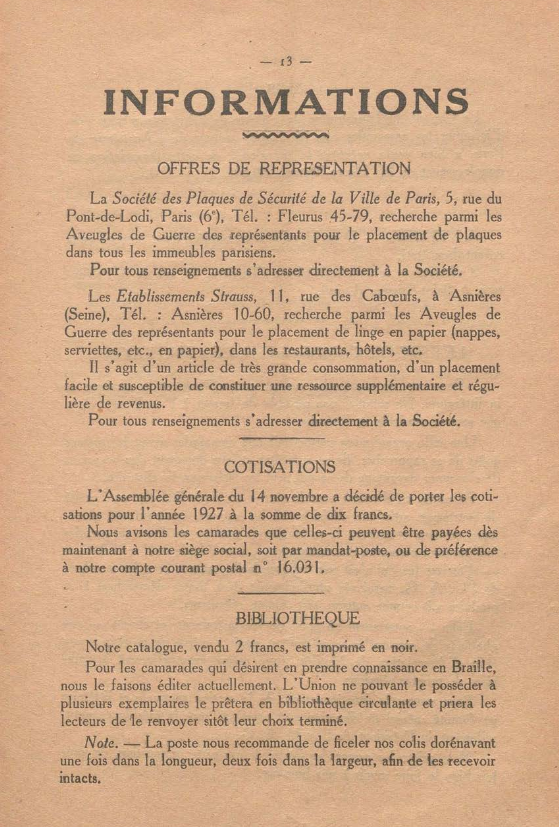
\includegraphics[width=0.4\linewidth]{images/doc12252_page15.png}
  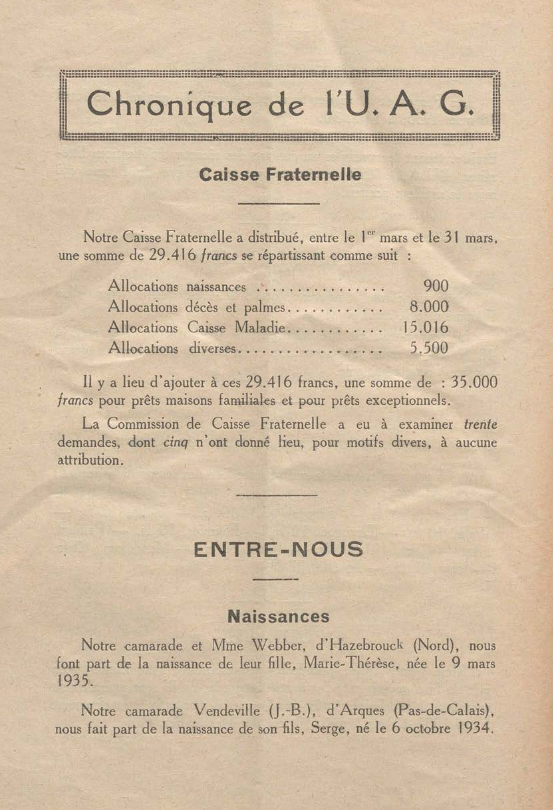
\includegraphics[width=0.403\linewidth]{images/doc12295_page20.png}
  \caption{\textit{Bulletin mensuel de l’Union des Aveugles de guerre et du Journal des blessés aux yeux}, édition de janvier 1927 (page 15, gauche) et avril 1935 (page 20, droite).}
  \label{fig:bulletin_uag}
  \vspace{-.5cm}
\end{figure}

\begin{figure}[htp]
  \centering
  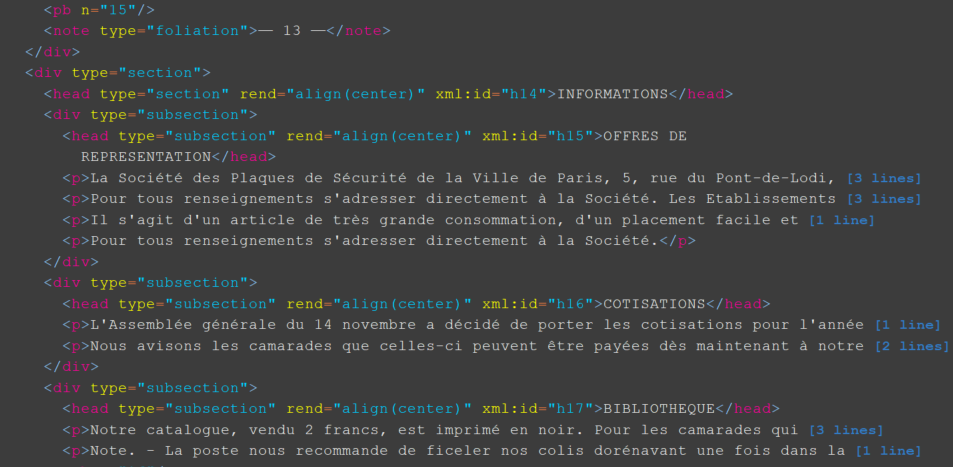
\includegraphics[width=0.88\linewidth]{images/doc12252_page15_xml.png}
  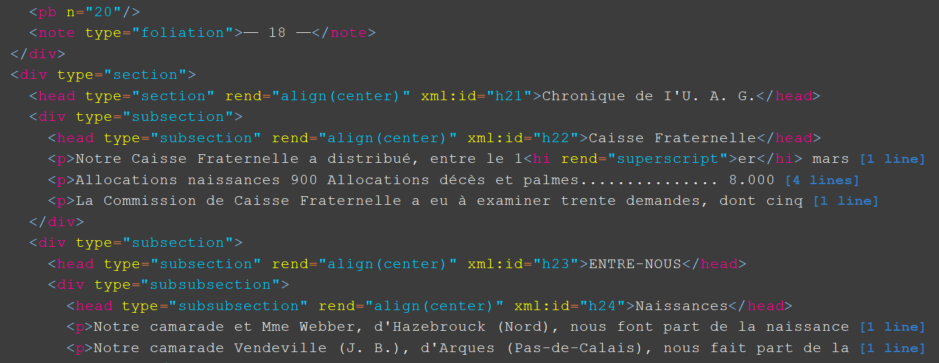
\includegraphics[width=0.88\linewidth]{images/doc12295_page20_xml.png}
  \caption{Encodage XML-TEI des pages de 1927 (haut) et 1935 (bas) présentées dans la figure~\ref{fig:bulletin_uag}.}
  \label{fig:xml_encoding}
  \vspace{-.6cm}
\end{figure}

\subsection{Adapter le \textit{chunking} pour le RAG à l’encodage XML-TEI}
Un point crucial dans l’implémentation d’un système RAG est la segmentation documentaire (\textit{chunking}), c’est-à-dire la façon dont les documents sont découpés en unités qui seront indexées, recherchées et fournies au modèle génératif. Les stratégies classiques consistent à découper les textes en segments fixes, mais cette approche fragmente souvent le contexte et affaiblit la cohérence sémantique des passages récupérés. Des travaux récents examinent des alternatives pour améliorer ce processus. Par exemple, la comparaison des techniques de \textit{late chunking} et de \textit{contextual retrieval}, montre que la récupération enrichie par le contexte, bien que plus coûteuse en calcul, préserve mieux l’intégrité sémantique~\cite{merola_reconstructing_2025}.

D’autres travaux s’intéressent plus spécifiquement à la relation entre la structure des documents et les stratégies de segmentation. Les auteurs de \cite{lu_hichunk_2025} proposent une approche de \textit{chunking} hiérarchique, fondée sur l’idée que les documents possèdent une organisation multiniveaux qui peut être exploitée pour définir des unités de récupération de granularité variable. Leur méthode vise à respecter la structure interne des documents afin d’améliorer la récupération dans les systèmes RAG, indépendamment du domaine ou du format de représentation.
Dans le cas de notre expérience, nous avons décidé de structurer le \textit{chunking} en utilisant les balises structurelles présentes dans notre corpus, afin d’extraire les métadonnées pour compléter le mécanisme de \textit{retrieval}.

\section{Quand le texte encodé devient texte généré : méthodes et résultats}
\subsection{Implémentation et paramétrage du système RAG}
Pour implémenter le système RAG, nous avons développé une interface interactive à l'aide de Streamlit\footnote{\url{https://streamlit.io}.}, permettant une manipulation flexible du corpus et des paramètres du système. Le pipeline repose sur LlamaIndex~\cite{Liu_LlamaIndex_2022} pour l'orchestration de l'indexation et de la récupération, et sur le modèle d'\textit{embeddings} \textit{intfloat/multilingual-e5-large}~\cite{wang2024multilingual}, choisi pour ses performances sur des textes français et multilingues de registres variés. Plusieurs LLM \textit{open source} ont été intégrés pour la génération, notamment \textit{Mistral-7B-Instruct}\footnote{\url{https://huggingface.co/mistralai/Mistral-7B-Instruct-v0.1}.} et \textit{Zephyr-7B}~\cite{tunstall2023zephyr}, afin de ne pas dépendre d'API propriétaires. L'interface expose les paramètres principaux : 
\begin{itemize} 
    \item le top-k\footnote{Nombre de passages récupérés soumis au modèle.};
    \item la température\footnote{Paramètre du modèle de langage qui influence la diversité des réponses générées.}; 
    \item le nombre maximal de tokens générés;
    \item le mode "\textit{retrieval only}" \footnote{Interrogation directe de l'index sans passer par la génération.};
    \item des filtres post-récupération\footnote{Affinage des résultats par date, type de \textit{chunk} ou mots-clés présents dans les métadonnées.}.
\end{itemize}

Le point central du pipeline est la stratégie de \textit{chunking}, entièrement pilotée par la structure TEI du corpus. Un module de détection automatique analyse par échantillonnage aléatoire un sous-ensemble de fichiers XML pour déterminer, sans intervention manuelle, le type documentaire majoritaire du corpus — correspondance, édition littéraire, édition parallèle, etc. — ainsi que la granularité de découpage appropriée. La décision repose sur une taxonomie des balises \texttt{<div>} selon leur rôle : unité de \textit{chunk} directe (par exemple \texttt{<div type="chapter">} ou \texttt{<div type="letter">}), conteneur récursif à traverser (par exemple \texttt{<div type="section">}), ou élément à ignorer (pages de titre, tables des matières). La densité tokenique moyenne par unité est ensuite mesurée : si elle dépasse un seuil de 400 tokens, le module active une décomposition au niveau des \texttt{<p>} ; si un paragraphe individuel dépasse encore ce seuil, il est soumis à un découpage par phrase. Cette cascade à trois niveaux garantit que chaque \textit{chunk} reste dans une plage cohérente pour l'encodage sémantique, quelle que soit la structure interne du corpus. Enfin, les métadonnées extraites du \texttt{<teiHeader>} — auteur, date, titre de section, type de division — sont propagées vers chaque \textit{chunk}, ce qui permet à la fois d'afficher des sources traçables dans l'interface et d'alimenter les filtres post-récupération.

\subsection{Des résultats prometteurs et particulièrement détaillés}
Afin d’évaluer le fonctionnement du RAG\footnote{\url{https://github.com/obtic-sorbonne/rag-humanistica}.}, expérimenté sur le corpus AVH contenant 284 fichiers et représentant 27 609 \textit{chunks}, plusieurs questions de nature variée ont été soumises au système. L’ensemble de ces questions et réponses est présenté en annexe \ref{appdx:questions_rag}. Les résultats obtenus montrent que le RAG fournit, de manière générale, des réponses claires et pertinentes. Il restitue fidèlement les informations présentes dans les documents sources (en mentionnant le document cité) ou, lorsque la question est formulée de manière plus large, il est capable d’en proposer une extrapolation raisonnée.
Par ailleurs, le RAG démontre une bonne constance dans ses réponses. En effet, comme l’illustre le tableau \ref{appdx:requetesdoubles}, lorsqu’une même question est posée à plusieurs reprises, les réponses produites sont similaires, voire identiques, tout comme les documents à partir desquels les informations sont récupérées. En outre, le système se distingue par sa capacité à ne pas produire d’informations infondées : lorsqu’une réponse ne peut être établie à partir des documents disponibles, le RAG n’invente pas de contenu et mentionne l’absence de résultat trouvé (\ref{appdx:requetesnonpertinentes}).
L’intérêt principal du RAG proposé, ainsi que du \textit{chunking} adopté, est notamment mis en évidence par les résultats détaillés figurant en annexe \ref{appdx:details_rag}. Ces résultats montrent en particulier que le \textit{chunking} hiérarchique s’avère pertinent, dans la mesure où il permet d’identifier les réponses les plus adaptées au sein de différents types de sections (Annexe \ref{appdx:details_rag} Figure \ref{appdx:retourgeneral}).
De plus, dans les retours détaillés par source (Annexe \ref{appdx:details_rag} Figure \ref{appdx:retourparsource}), le RAG a été conçu de façon à fournir des informations contextuelles supplémentaires, notamment le type et le titre de la section dont la réponse a été extraite. Ce choix facilite ultérieurement la recherche de l’information dans le fichier XML correspondant. 

\section{Une solution fonctionnelle à renforcer, généraliser, déployer…}
\subsection{Renforcer les capacités du RAG}
La solution proposée repose actuellement sur un fonctionnement essentiellement extractif, dans lequel les réponses générées correspondent à des informations explicitement présentes dans le corpus. Une première perspective d’amélioration consisterait à doter le RAG de capacités de raisonnement, lui permettant de traiter des questions nécessitant une inférence ou une agrégation d’informations distribuées dans plusieurs documents. Il deviendrait ainsi possible de formuler des requêtes transversales, par exemple de nature quantitative ou comparative, impliquant la combinaison de données issues de différentes entités ou sections du corpus. 

Une autre piste d’amélioration concerne l’évaluation de modèles de langage de plus grande taille. Des modèles disposant de gestion du contexte plus avancée pourraient améliorer la qualité des réponses, en particulier pour des requêtes complexes mobilisant plusieurs unités de contexte. Une telle exploration permettrait de mieux mesurer l’impact du choix du modèle sur l’exploration d’éditions numériques structurées et d’identifier des compromis adaptés aux contraintes des projets en humanités numériques. 


\subsection{Généraliser l’approche à d’autres types d’encodage TEI}
L’expérience que nous présentons ici n’est qu’un simple \textit{proof-of-concept}, l’idée ayant été de voir, avec un encodage basique et simplement structuré, si une édition numérique en TEI pouvait devenir mémoire de RAG. Si cela a effectivement été concluant, il est cependant essentiel d'approfondir notre recherche, pour garantir sa généralisation à d’autres types d’encodages. La TEI se caractérise par une quantité importante de balises et d’attributs, adaptés surtout aux types de documents travaillés, et il serait pertinent de vérifier que le \textit{chunking} fonctionne aussi bien pour d’autres corpus. 
Un premier élément de réponse peut être apporté avec des tests que nous avons effectués sur deux autres corpus TEI, une correspondance de la Première Guerre mondiale\footnote{1 492 fichiers, 21 111 chunks.}~\cite{chiffoleau:hal-03628094}, et des documents relatant l’Holocauste\footnote{279 fichiers, 11 588 chunks.}~\cite{beniere:hal-04594190}. Comme le montrent les annexes \ref{appdx:questions_rag_pec} et \ref{appdx:questions_rag_ehri}, le RAG semble répondre aussi bien qu’avec le corpus initial, ce qui est encourageant pour son adaptation à d’autres corpus TEI. 

\subsection{Déployer le RAG au sein d’une instance de publication de l’édition numérique}
Enfin, au regard du projet même sur lequel s’est appuyé le RAG pour mettre en place sa mémoire, la finalité de cette édition numérique est de la déployer sur un site web pour donner accès à tous aux collections patrimoniales. L'intérêt majeur de cette édition étant d’être accessible pour tous et notamment les principaux concernés par ces documents, le RAG pourrait être d’une grande utilité pour pouvoir faire des recherches dans les collections sans connaître ou voir son contenu. Il sera donc nécessaire de réfléchir aux systèmes de gestions de contenus (CMS) qui existent pour découvrir si et comment cela pourrait s’intégrer, afin de proprement combiner les deux.

\section*{Conclusion}
Dans ce papier, nous avons montré qu’il était possible d’utiliser l’encodage XML-TEI d’éditions scientifiques numériques, comme mémoire pour un système RAG, utilisant donc la TEI comme outil de médiation entre une édition numérique et un RAG, augmentant ainsi ses capacités d’exploitation.
Nos tests supplémentaires nous ont permis d’entrevoir que la technique pouvait effectivement s’adapter à d’autres corpus TEI, sans avoir à initier de changements trop conséquents sur la structure même du RAG. Il sera nécessaire néanmoins de l’appliquer à une plus grande quantité et diversité de fonds, pour tester de manière plus approfondie ses compétences et ses limites.


% Imprime la bibliographie à la fin. Gardez cette ligne après le texte
% principal de votre article et avant une annexe.

\printbibliography

\bigskip

% Vous pouvez inclure une annexe en utilisant la commande suivante
\appendix
\section{Le prompt du RAG} \label{appdx:prompt} 
\begin{tcolorbox}[
  colback=purple!6,        % fond pastel (modifiable)
  colframe=black,        % bord noir
  boxrule=0.8pt,         % épaisseur du cadre
  arc=0mm,               % coins légèrement arrondis
  left=6pt,
  right=6pt,
  top=6pt,
  bottom=6pt,
  fontupper=\ttfamily,   % police monospace
]
Tu es un assistant spécialisé dans les éditions numériques en humanités.\\
Réponds uniquement en te basant sur les documents fournis.\\
Cite toujours tes sources avec la date et le titre du document.
\end{tcolorbox}

\bigskip


\section{Les requêtes faites au RAG (Corpus AVH)} \label{appdx:questions_rag} 
\subsection{Cohérence des réponses lors de répétitions de questions} \label{appdx:requetesdoubles}
\paragraph{Question :} Peux-tu me citer les naissances en 1921?

\paragraph{Réponse (Version 1) :}
\begin{enumerate}
    \item Notre camarade et Mme Sibiril (Pierre), nous font part de la naissance de leur fille Suzanne, née le 2 octobre 1921.
    \item Notre camarade et Mme Colleuille (Maurice), nous font part de la naissance de leur fils Robert-Maurice, né le 8 septembre.
    \item Notre camarade et Mme Felgeirolles (Henri), nous font part de la naissance de leur fille Marie-Louise, née le 30 août.
    \item Notre camarade et Mme Fossati (André), nous font part de la naissance de leur fils Maurice, né le 27 septembre.
    \item Notre camarade et Mme Rascle (Edmond), nous font part de la naissance de leur fille Raymonde, née le 4 octobre.
    \item Notre camarade et Mme Malgoire, nous font part de la naissance de leur enfant, né le 24 septembre.
    \item Notre camarade et Mme Rouxel (E.), nous font part de la naissance de leur fille Blanche, née le 7 octobre.
    \item Notre camarade et Mme Beve (E.), nous font part de la naissance de leur fille Marthe, née le 22 octobre.
    \item Notre camarade et Mme Lamaury (Pierre), nous font part de la naissance de leur fils Fernand.
    \item Notre camarade et Mme Hassen Ben Salem Kraiem, nous font pa. de la naissance de leur fille, née le 20 octobre.
    \item Notre camarade et Mme Boucher, nous font part de la naissance de leur fils Raymond, né le 27 octobre 1921.
    \item Notre camarade et Mme Gambert (François), nous font part de la naissance de leur deuxième garçon, né le 22 septembre.
    \item Notre camarade et Mme Moteau (Jean), nous font part de la naissance de leur deuxième garçon, né le 17 octobre.
\end{enumerate}

\paragraph{Réponse (Version 2) :}
\begin{enumerate}
    \item Notre camarade et Mme Sibiril (Pierre) ont eu une fille Suzanne le 2 octobre 1921.
    \item Notre camarade et Mme Colleuille (Maurice) ont eu un fils Robert-Maurice le 8 septembre.
    \item Notre camarade et Mme Felgeirolles (Henri) ont eu une fille Marie-Louise le 30 août.
    \item Notre camarade et Mme Fossati (André) ont eu un fils Maurice le 27 septembre.
    \item Notre camarade et Mme Rascle (Edmond) ont eu une fille Raymonde le 4 octobre.
    \item Notre camarade et Mme Malgoire ont eu un enfant le 24 septembre.
    \item Notre camarade et Mme Moteau (Jean) ont eu un deuxième garçon le 17 octobre.
    \item Notre camarade et Mme Beve (E.) ont eu une fille Marthe le 22 octobre.
    \item Notre camarade et Mme Lamaury (Pierre) ont eu un fils Fernand.
    \item Notre camarade et Mme Hassen Ben Salem Kraiem ont eu une fille le 20 octobre.
    \item Notre camarade et Mme Boucher ont eu un fils Raymond le 27 octobre 1921.
    \item Notre camarade et Mme Gambert (François) ont eu leur deuxième garçon le 22 septembre.
    \item Notre camarade et Mme Rouxel (E.) ont eu une fille Blanche le 7 octobre.
    \item Notre camarade et Mme Lassalle (Auguste) ont eu une fille Augusta le 17 septembre.
    \item Notre camarade et Mme Denos (Jean) ont eu un fils Pierre le 14 octobre.
    \item Notre camarade et Mme Juif (Georges) ont eu une fille.
    \item Notre camarade et Mme Masson (François) ont eu un fils Louis le 8
\end{enumerate}

\separation

\paragraph{Question :} Qu'est-ce que la guerre ?

\paragraph{Réponse (Version 1) :}
\begin{enumerate}
\item La guerre est une action extérieure occasionnée par des événements de guerre et du fait de l'ennemi qui résulte en lésions graves et la destruction des vies humaines précieuses et des foyers (Bulletin mensuel de l'Union des aveugles de guerre et Journal des soldats blessés aux yeux - 17ème année 1935, n°2). 
\item Selon l'Union des aveugles de guerre, la guerre offensive est immorale et criminelle (Bulletin mensuel de l'Union des aveugles de guerre et Journal des soldats blessés aux yeux - 13ème année 1931, n°7). 
\end{enumerate}

\paragraph{Réponse (Version 2) :}
\begin{enumerate}
\item La guerre est l'action extérieure qui occasionne des lésions physiques à un individu pendant des événements de guerre et du fait de l'ennemi. (Source: Bulletin mensuel de l'Union des aveugles de guerre et Journal des soldats blessés aux yeux - 17ème année 1935, n°2) 
\item Quelle est la position de l'organisme sur la guerre offensive ? La guerre offensive est immorale et criminelle. (Source: Bulletin mensuel de l'Union des aveugles de guerre et Journal des soldats blessés aux yeux - 13ème année 1931, n°7)
\end{enumerate}

\subsection{Qualité des réponses à des questions diverses} \label{appdx:requetesdiverses}
\paragraph{Question :} Qu'est-ce que le vélo-car ?

\paragraph{Réponse :} The Vélocar is a bicycle that is car-like in appearance, with a structure that resembles a small automobile. It is propelled by pedaling, and it has three gears that allow it to reach speeds of up to 50 kilometers per hour and climb hills easily. The occupants pedal at their own pace, each with their own independent pedal and free wheel. (1927-12-01, Bulletin mensuel de l'Union des aveugles de guerre et Journal des soldats blessés aux yeux - 9ème année 1927 n°10)

\separation

\paragraph{Question :} Qu'est-ce qu'un aveugle de guerre ?

\paragraph{Réponse :}
According to the "Bulletin mensuel de l'Union des aveugles de guerre et Journal des soldats blessés aux yeux - 5ème année 1923, n°3" on 1923-03-01, an aveugle de guerre is not an invalid, but a mutilé; the difference is great. He is a man who, by virtue of a worldwide catastrophe, has lost the use of one of his senses, but who has not lost his intelligence, activity, skill, and the memory of everything he has seen. He can compensate for the sudden loss of his sight through new tactile and auditory"

\separation

\paragraph{Question :} La vie ...

\paragraph{Réponse :}
The life of the blind veterans is discussed in the documents, particularly their pensions, rehabilitation, employment, and social aide. For example, in the document "Bulletin mensuel de l'Union des aveugles de guerre et Journal des soldats blessés aux yeux - 5ème année 1923, n°1", there is a questionnaire about Franceville, a home for the blind veterans ...

\subsection{Neutralité pour des questions non pertinentes} \label{appdx:requetesnonpertinentes}
\paragraph{Question :} Qui a volé l'orange du marchand ?

\paragraph{Réponse :} The document does not provide information about someone stealing an orange from a merchant.

\separation

\paragraph{Question :} Qu'est-ce que l'iphone ?

\paragraph{Réponse :} L'iphone n'est pas mentionné dans les documents fournis, il est impossible de répondre à la question avec précision en se basant sur les documents.

\section{Détails des retours de requêtes (Corpus AVH)} \label{appdx:details_rag}
\begin{figure}[h!]
  \centering
  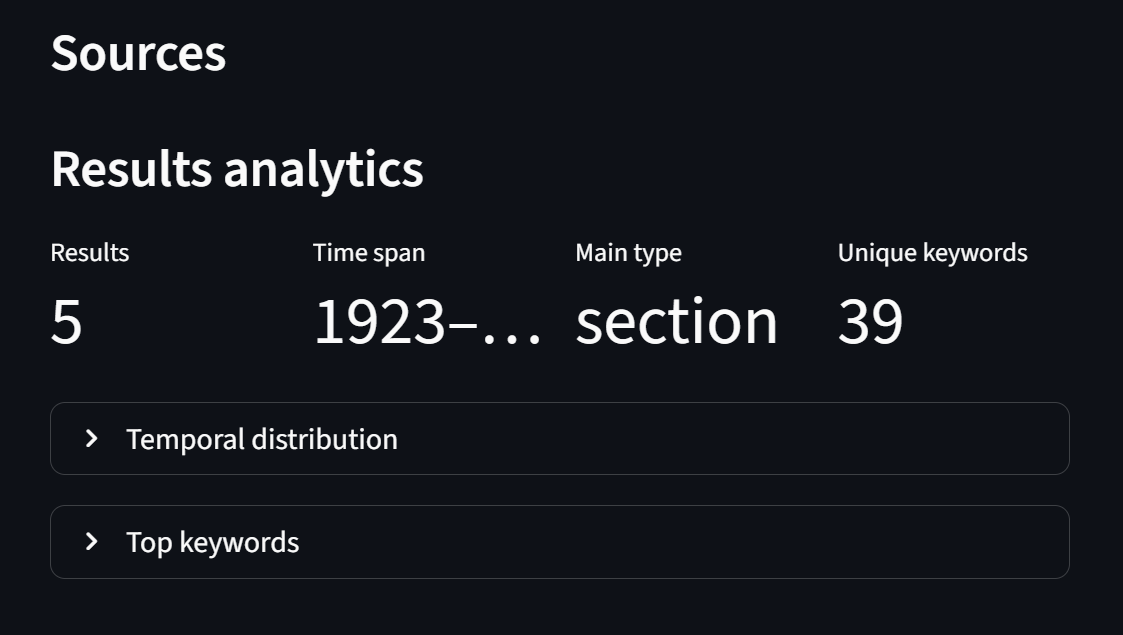
\includegraphics[width=0.8\linewidth]{images/analytics_1.png}
  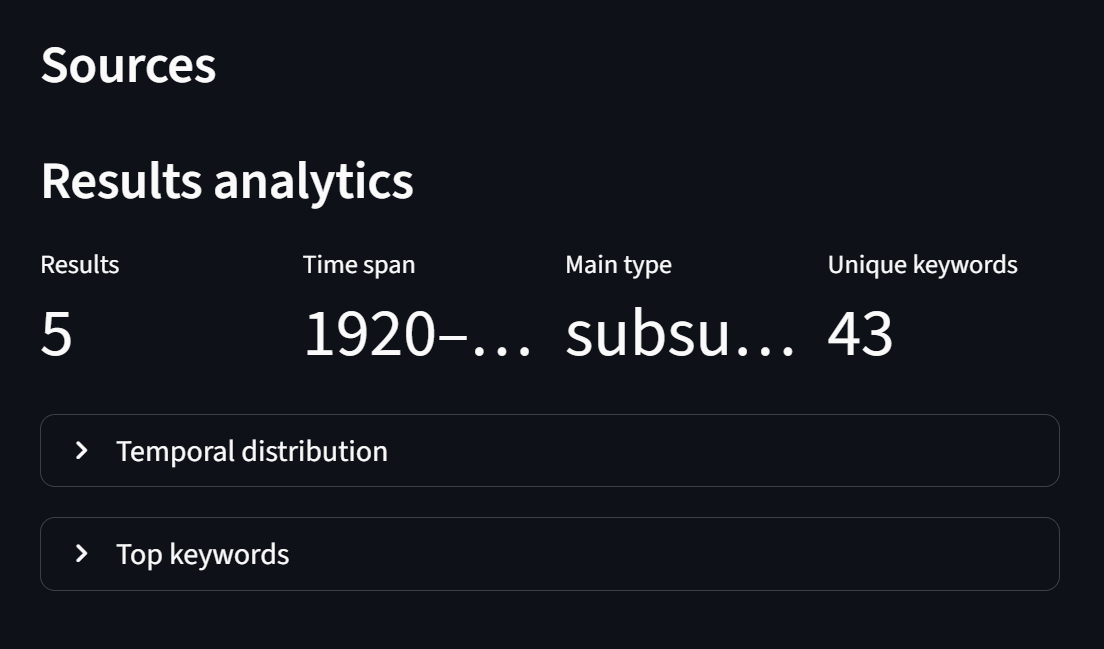
\includegraphics[width=0.8\linewidth]{images/analytics_2.png}
  \caption{Retour général après requête}
  \label{appdx:retourgeneral}
\end{figure}

\begin{figure}[p!]
  \centering
  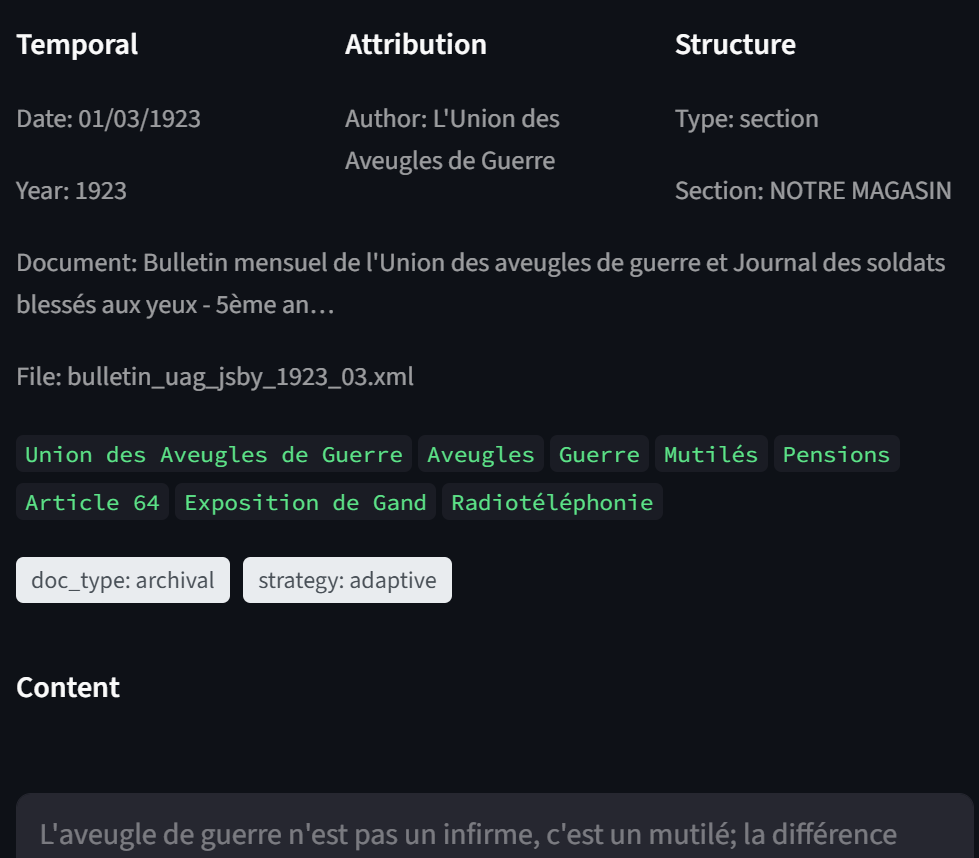
\includegraphics[width=0.6\linewidth]{images/details_1.png}
  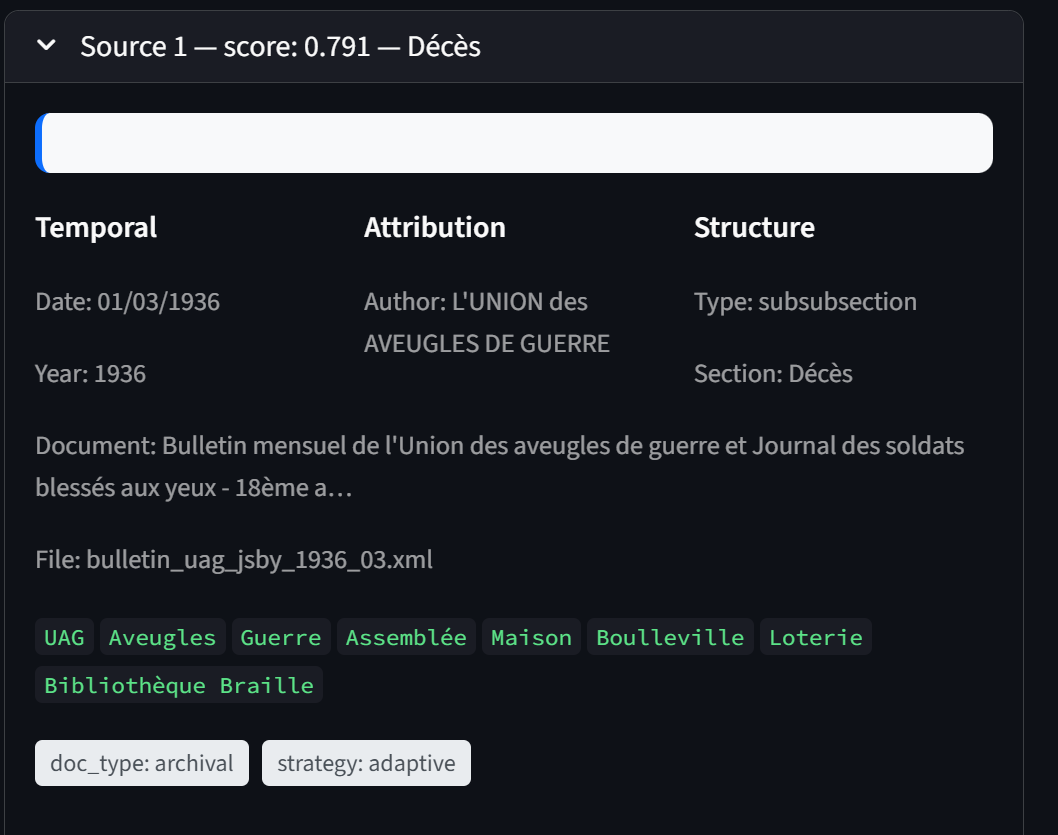
\includegraphics[width=0.6\linewidth]{images/details_2.png}
  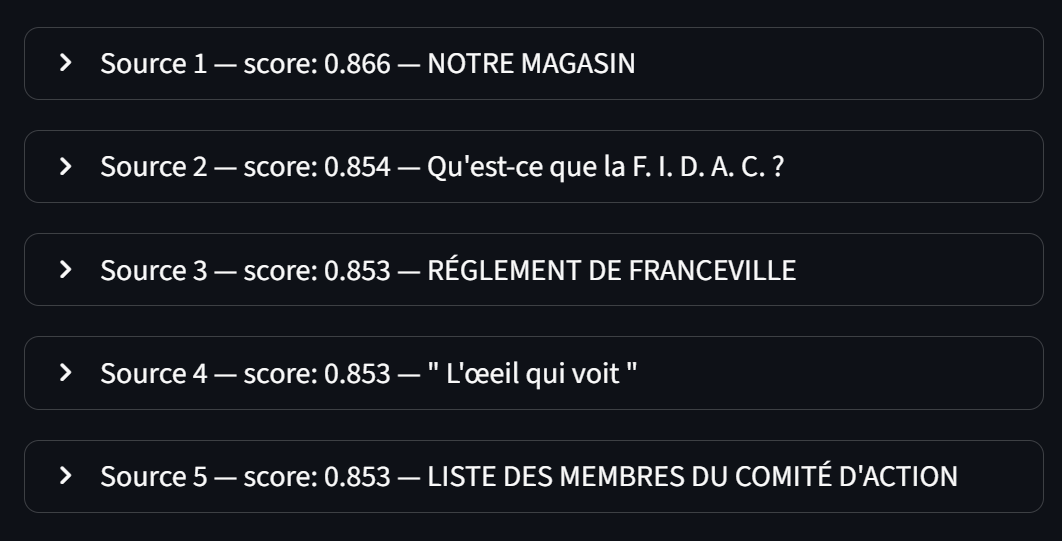
\includegraphics[width=0.6\linewidth]{images/details_3.png}
  \caption{Retour par source après requête}
  \label{appdx:retourparsource}
\end{figure}

\newpage
\section{Les requêtes faites au RAG (Corpus Paul d'Estournelles)} \label{appdx:questions_rag_pec} 
\bigskip
\paragraph{Question : } Comment s'appelle la fille de Paul d'Estournelles

\paragraph{Réponse}
The daughter of Paul d'Estournelles is named Henriette. \\ Reference(s): - doc\_title: Letter number 850 from Paul d'Estournelles de Constant to Nicholas Murray Butler (June 23, 1921) - file\_name: Lettre0850\_23juin1921.xml

\separation

\paragraph{Question : } Les Italiens

\paragraph{Réponse : }
\begin{enumerate}
    \item Les Italiens ont été irrités contre les Français, les Anglais et les Américains (Letter number 724 from Paul d'Estournelles de Constant to Nicholas Murray Butler, November 26, 1920).
    \item Les Italiens ont reçu une acclamation pour le fascisme, qui réclame la Dalmatie, l'Adriatique, la Méditerranée, Nice, la Savoie, la Corse, la Tunisie, une partie de la Suisse, etc., et a tendu la main au féodalisme Hongrois contre les Slaves des Balkans (Letter number 1206 from Paul d'Estournelles de Constant to Nicholas Murray Butler, November 29, 1922).
    \item Les Italiens ne disent rien ni de Trieste, ni du Trentin, mais pensent aux sacrifices dont ils faut payer pour aboutir à des succès actuels. Ils ont également souligné que si les Allemands envahissent de nouveau la Péninsule, il n'est pas clair de savoir si il est la peine de se ruiner pour aboutir à ce résultat (Letter number 713 from Paul d'Estournelles de Constant to Nicholas Murray Butler, October 19, 1920).
\end{enumerate}

\separation

\paragraph{Question : } Qui est Elihu Root ?

\paragraph{Réponse : } Elihu Root is a person who is mentioned in the letters from Paul d'Estournelles de Constant to Nicholas Murray Butler, specifically in the documents "Letter number 1451 from Paul d'Estournelles de Constant to Nicholas Murray Butler (December 4, 1923)" and "Letter number 1438 from Paul d'Estournelles de Constant to Nicholas Murray Butler (November 22, 1923)". \\ 
Elihu Root was a prominent American statesman, lawyer, and academic who served as the United States Secretary of War and Secretary of State. He was also the President of the Carnegie Endowment for International Peace. \\
Reference(s): - "Letter number 1451 from Paul d'Estournelles de Constant to Nicholas Murray Butler (December 4, 1923)", 1957 - "Letter number 1438 from Paul d'Estournelles de Constant to Nicholas Murray Butler (November 22, 1923)", 1957

\separation

\paragraph{Question}
Prix Nobel de la Paix

\paragraph{Réponse}
Based on the provided documents, the Nobel Peace Prize is not directly mentioned. However, in letter number 407 from Paul d'Estournelles de Constant to Nicholas Murray Butler dated August 9, 1918, it is mentioned that the Carnegie Endowment for International Peace is offering its services to the U.S. government to help treat international affairs related to the war. This organization was established by Andrew Carnegie, who received the Nobel Peace Prize in 1911. (1957, 1957)

\separation

\paragraph{Question : } Traité de Versailles

\paragraph{Réponse : }
\begin{enumerate}
    \item The Treaty of Peace has been proclaimed and it will have to become a reality. (Letter number 14 from Paul d'Estournelles de Constant to Nicholas Murray Butler, December 3, 1914)
    \item The Treaty of Versailles has been signed, but it remains to be applied and amended in such a way that this war truly ends and cannot resume. (Letter number 622 from Paul d'Estournelles de Constant to Nicholas Murray Butler, February 15, 1920)
    \item The Treaty of Peace, as it was proclaimed in a letter from Paul d'Estournelles de Constant to Nicholas Murray Butler on December 3, 1914 \\ (ref. Lettre0014\_3decembre1914.xml).
    \item The Treaty of Versailles, which was signed but not yet executed, according to a statement in a letter from Paul d'Estournelles de Constant to Nicholas Murray Butler on September 18, 1923 (ref. Lettre1391\_18septembre1923.xml).
    \item The Treaty of Versailles, which Germany has signed but is yet to be applied and amended to ensure the cessation of the war in a letter from Paul d'Estournelles de Constant to Nicholas Murray Butler on February 15, 1920 (ref. Lettre0622\_15fevrier1920.xml).
    \item The Treaty of Versailles, which Germany has accepted without conditions in a letter from Paul d'Estournelles de Constant to Nicholas Murray Butler on June 24, 1919 (ref. Lettre0552\_24juin1919.xml).
\end{enumerate}

\bigskip 

\section{Les requêtes faites au RAG (Corpus EHRI)} \label{appdx:questions_rag_ehri} 
\bigskip
\paragraph{Question : } La déportation des Juifs vers Auschwitz

\paragraph{Réponse : } Les textes fournis décrivent des déportations de Juifs vers Auschwitz-Birkenau. Les témoignages de Otto Kalwo et Eduard de Wind font mention de cette destination. (Documents EHRI-DC-054\_DE\_EN.xml et EHRI-DC-066\_DE\_EN.xml)

\separation

\paragraph{Question : } Comment est la vie dans le ghetto de terezin ?

\paragraph{Réponse : } La vie dans le ghetto de Terezin était difficile. Les barracks étaient surpeuplés, une grande partie des ghettoisés devaient dormir sur le sol, car tout espace était utilisé comme lieu de sommeil. Sans lits, sans matelas ou sacs à paillasses, seulement quelques-uns étaient temporairement disponibles. Les campagnards dormaient sur des sols froids, beaucoup d'entre eux dans des salles telles que les écuries, les entrepôts et les lieux similaires sur le sol de ciment dur. Dans les baraques des Sudè

\separation

\paragraph{Question : } attaque antisémite violente

\paragraph{Réponse : } The documents provide multiple evidence of violent anti-Semitic attacks in Slovakia. In the memorandum by the Association of the Victims of Racial Persecution Košice chapter, they mention anti-Jewish riots (doc\_title: Memorandum on anti-Jewish riots in Slovakia, Memorandum zu antijüdischen Ausschreitungen in der Slowakei, Memorandum o protižidovských nepokojích na Slovensku, paragraph xml\_id: ). Furthermore, the Association of the Victims of Racial Persecution, eastern district of Košice, ...

\separation

\paragraph{Question : } hitler

\paragraph{Réponse : } The query "hitler" does not appear in the provided documents.

\separation

\paragraph{Question}
Aggression non juive

\paragraph{Réponse}
At the personal level, the persecution is even more severe. Association with Germans is strictly forbidden, and even kids are not allowed to play with German kids. Although in legal terms we are not expelled from the country, the method used goes against humanity and arouses (uncontrollable) anger. (Giuseppe Talamo Atenolfi on Hungarian actions against Jews in occupied Galicia in 1942, Giuseppe Talamo Atenolfi über ungarische Aktionen gegen Juden im besetzten Galizien im Jahr 1942, EHRI-DR-19

\separation

\paragraph{Question : } Aggression non-juive

\paragraph{Réponse : }
\begin{enumerate}
    \item In the document "A fifteen-year-old youth, on the German invasion of Wyszków and surrounding areas" written on an undetermined date, the author describes how Jews were severely beaten. (keywords: testimony, robberies, beaten) 
    \item In the document "Ray Atherton on the reaction of the non-Jewish Bulgarian population towards antisemitic demonstrations in 1939", the author mentions that there is no sympathy in Bulgaria for the antisemitic demonstrations of the organization "Workers of New Bulgaria" ...
\end{enumerate}

\separation

\paragraph{Question : } Qui est persecuté outre les juifs

\paragraph{Réponse : } Les juifs sont persecutés en plus de quelqu'un d'autre, mais il n'est pas spécifié dans les documents fournis qui sont les autres personnes qui sont persecutées.

\end{document}